\chapter{Analysis}\label{ch:5}

\begin{figure}[H]
    \centering
    \includegraphics[width = \textwidth]{Figures/p_ANN_learning.pdf}
    \caption{The learning process of the Artificial Neural Network.}
    \label{fig:p_learning_process_ANN}
\end{figure}


\begin{table}[H]
     \centering
     \caption{Confusion Matrix}
     \label{tab:Confusion_matrix}
     \begin{tabular}{@{}cc cc@{}}
     \multicolumn{1}{c}{} &\multicolumn{1}{c}{} &\multicolumn{2}{c}{\textbf{Actual}} \\
     \cmidrule(lr){3-4}
     \multicolumn{1}{c}{} & 
     \multicolumn{1}{c}{} & 
     \multicolumn{1}{c}{Default} & 
     \multicolumn{1}{c}{Not-default} \\
     \vspace{0.1cm}
     \cline{2-4}
     \multirow[c]{2}{*}{\rotatebox[origin=tr]{90}{\textbf{Predicted}}} & Default  & 196.712 & 1320 \\[1.5ex] & Not-default &631 & 5.460 \\ \cline{2-4}
     \end{tabular}
     \end{table}
\begin{table}[H]
     \centering
     \caption{Confusion Matrix}
     \label{tab:Confusion_matrix}
     \begin{tabular}{@{}cc cc@{}}
     \multicolumn{1}{c}{} &\multicolumn{1}{c}{} &\multicolumn{2}{c}{\textbf{Actual}} \\
     \cmidrule(lr){3-4}
     \multicolumn{1}{c}{} & 
     \multicolumn{1}{c}{} & 
     \multicolumn{1}{c}{Default} & 
     \multicolumn{1}{c}{Not-default} \\
     \vspace{0.1cm}
     \cline{2-4}
     \multirow[c]{2}{*}{\rotatebox[origin=tr]{90}{\textbf{Predicted}}} & Default  & 196.438&748 \\[1.5ex] & Not-default &905&6.032 \\ \cline{2-4}
     \end{tabular}
     \end{table}


\begin{figure}[H]
    \centering
    \includegraphics[width = \textwidth]{Figures/p_performance.pdf}
    \caption{Performance metrics of the models.}
    \label{fig:p_performance}
\end{figure}

\begin{figure}[H]
    \centering
    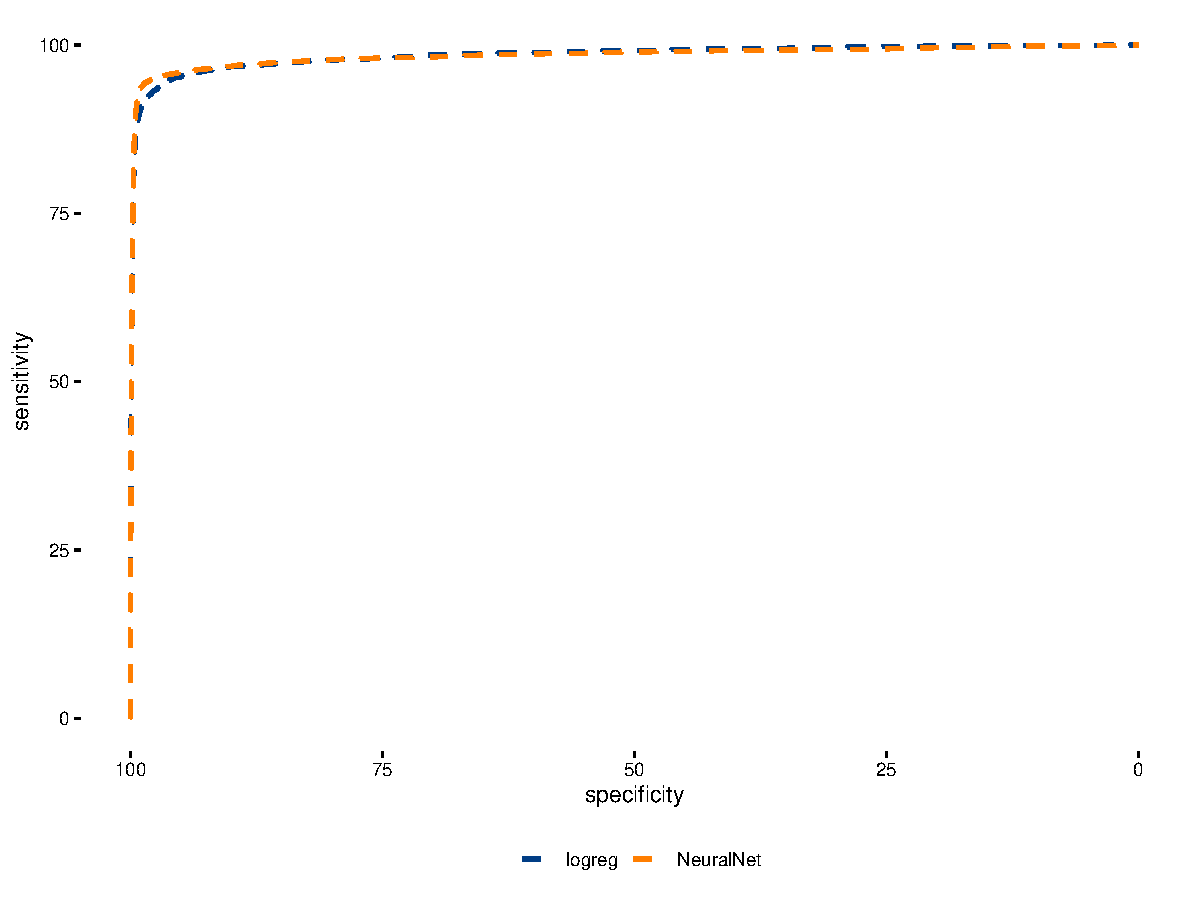
\includegraphics[width = \textwidth]{Figures/p_roc.pdf}
    \caption{ROC Curves of the two models.}
    \label{fig:p_roc}
\end{figure}


\begin{figure}[H]
    \centering
    \includegraphics[width = \textwidth]{Figures/p_lime_features_ANN.pdf}
    \caption{LIME - Feature importance of 10 cases in the held out testset.}
    \label{fig:LIME_Features}
\end{figure}

    \section{Default Prediction}
    
        \subsection{Class Imbalance}
        
        \subsection{Cost Sensitive Learning}
        
        \subsection{Model Architecture}
\begin{enumerate}
    \item How can financial institutions benefit from a more correct PD estimate?
    \begin{enumerate}
        \item Estimate a more correct captial requirement, and maybe decrease it dependent on the costumers. Thus, the financial institution is able to increase efficiency of its capital. 
        \item More correct Value at Risk, Expected Shortfall and such risk estimates. 
        \item and since we are able to trust the ANN due to the LIME algorithm we are also able to implement this in the financial industry.
    \end{enumerate}
    
    Overall increase the profit of the business.
\end{enumerate}